% -------------------------------- SVILUPPO -------------------------------------

% ---------------- RELAZIONE PROGETTO DI PROGRAMMAZIONE AD OGGETTI (OOP) --------
\documentclass[a4paper,12pt]{report}

% ----------------------------- PREAMBLE --------------------------------------- 

\usepackage{lmodern}
\usepackage{alltt, fancyvrb, url}
\usepackage{float}
\usepackage{graphicx}
\usepackage[utf8]{inputenc}
\usepackage{hyperref}
\usepackage{amsmath,amssymb,amsthm}

\usepackage[italian]{babel}

\usepackage[italian]{cleveref}

\usepackage{comment}
\usepackage{microtype}
\usepackage{fancyhdr}

\usepackage[scaled=.92]{helvet}
\usepackage[T1]{fontenc}

\usepackage{lscape}

\usepackage{subcaption}

% hyperref settings
\hypersetup{
	colorlinks=true,
	linkcolor=black, %blue
	filecolor=magenta,      
	urlcolor=cyan,
	pdftitle={Sharelatex Example},
	bookmarks=true,
	pdfpagemode=FullScreen,
}

% ----------------------------- PREAMBLE END -----------------------------------

\makeindex

\title{\textbf{Progetto di Tecnologie Web Report}}
\author{Luca Rengo | Alessandro Pioggia}

\begin{document}
	
	\makeatletter
	\begin{titlepage}
		\begin{center}
			
\includegraphics[width=0.7\linewidth]{Images/logo/alma_mater_studiorum_cesena_logo.png}\\[4ex]
			{\Huge  \@title }\\[3ex] 
			{\large  \@author}\\[3ex] 
			{\large \@date}
		\end{center}
	\end{titlepage}
	\makeatother
	\thispagestyle{empty}
	\newpage
	
	%\maketitle
	
	\tableofcontents

	\newpage
	
	% \input: import the commands from filename.tex to target file.
	
	% \include: does a \clearpage and does an \input.
	\section{Introduzione}
	\textsf{\small L'obiettivo del progetto è la realizzazione di un sito web riguardante un ristorante, \emph{Il Dojo dei Panini}, specializzato nella preparazione e vendita di panini gourmet su misura in tema Giappone.}
	\subsection{Dojo}
	\textsf{\small Il \emph{Dojo} è il luogo dove si svolgono le arti marziali, dal giapponese \emph{"Luogo dove si segue la via"}.}\\
	\textsf{\small I dojo erano spesso piccoli locali situati nelle vicinanze di un tempio o di un castello, ai margini delle foreste, in modo tale che i segreti delle tecniche venissero più facilmente preservati, allo stesso modo noi conserviamo da secoli, con cura e dedizione le ricette segrete per preparare i nostri panini.}\\
	
	\begin{figure}[ht] 
		\centering
		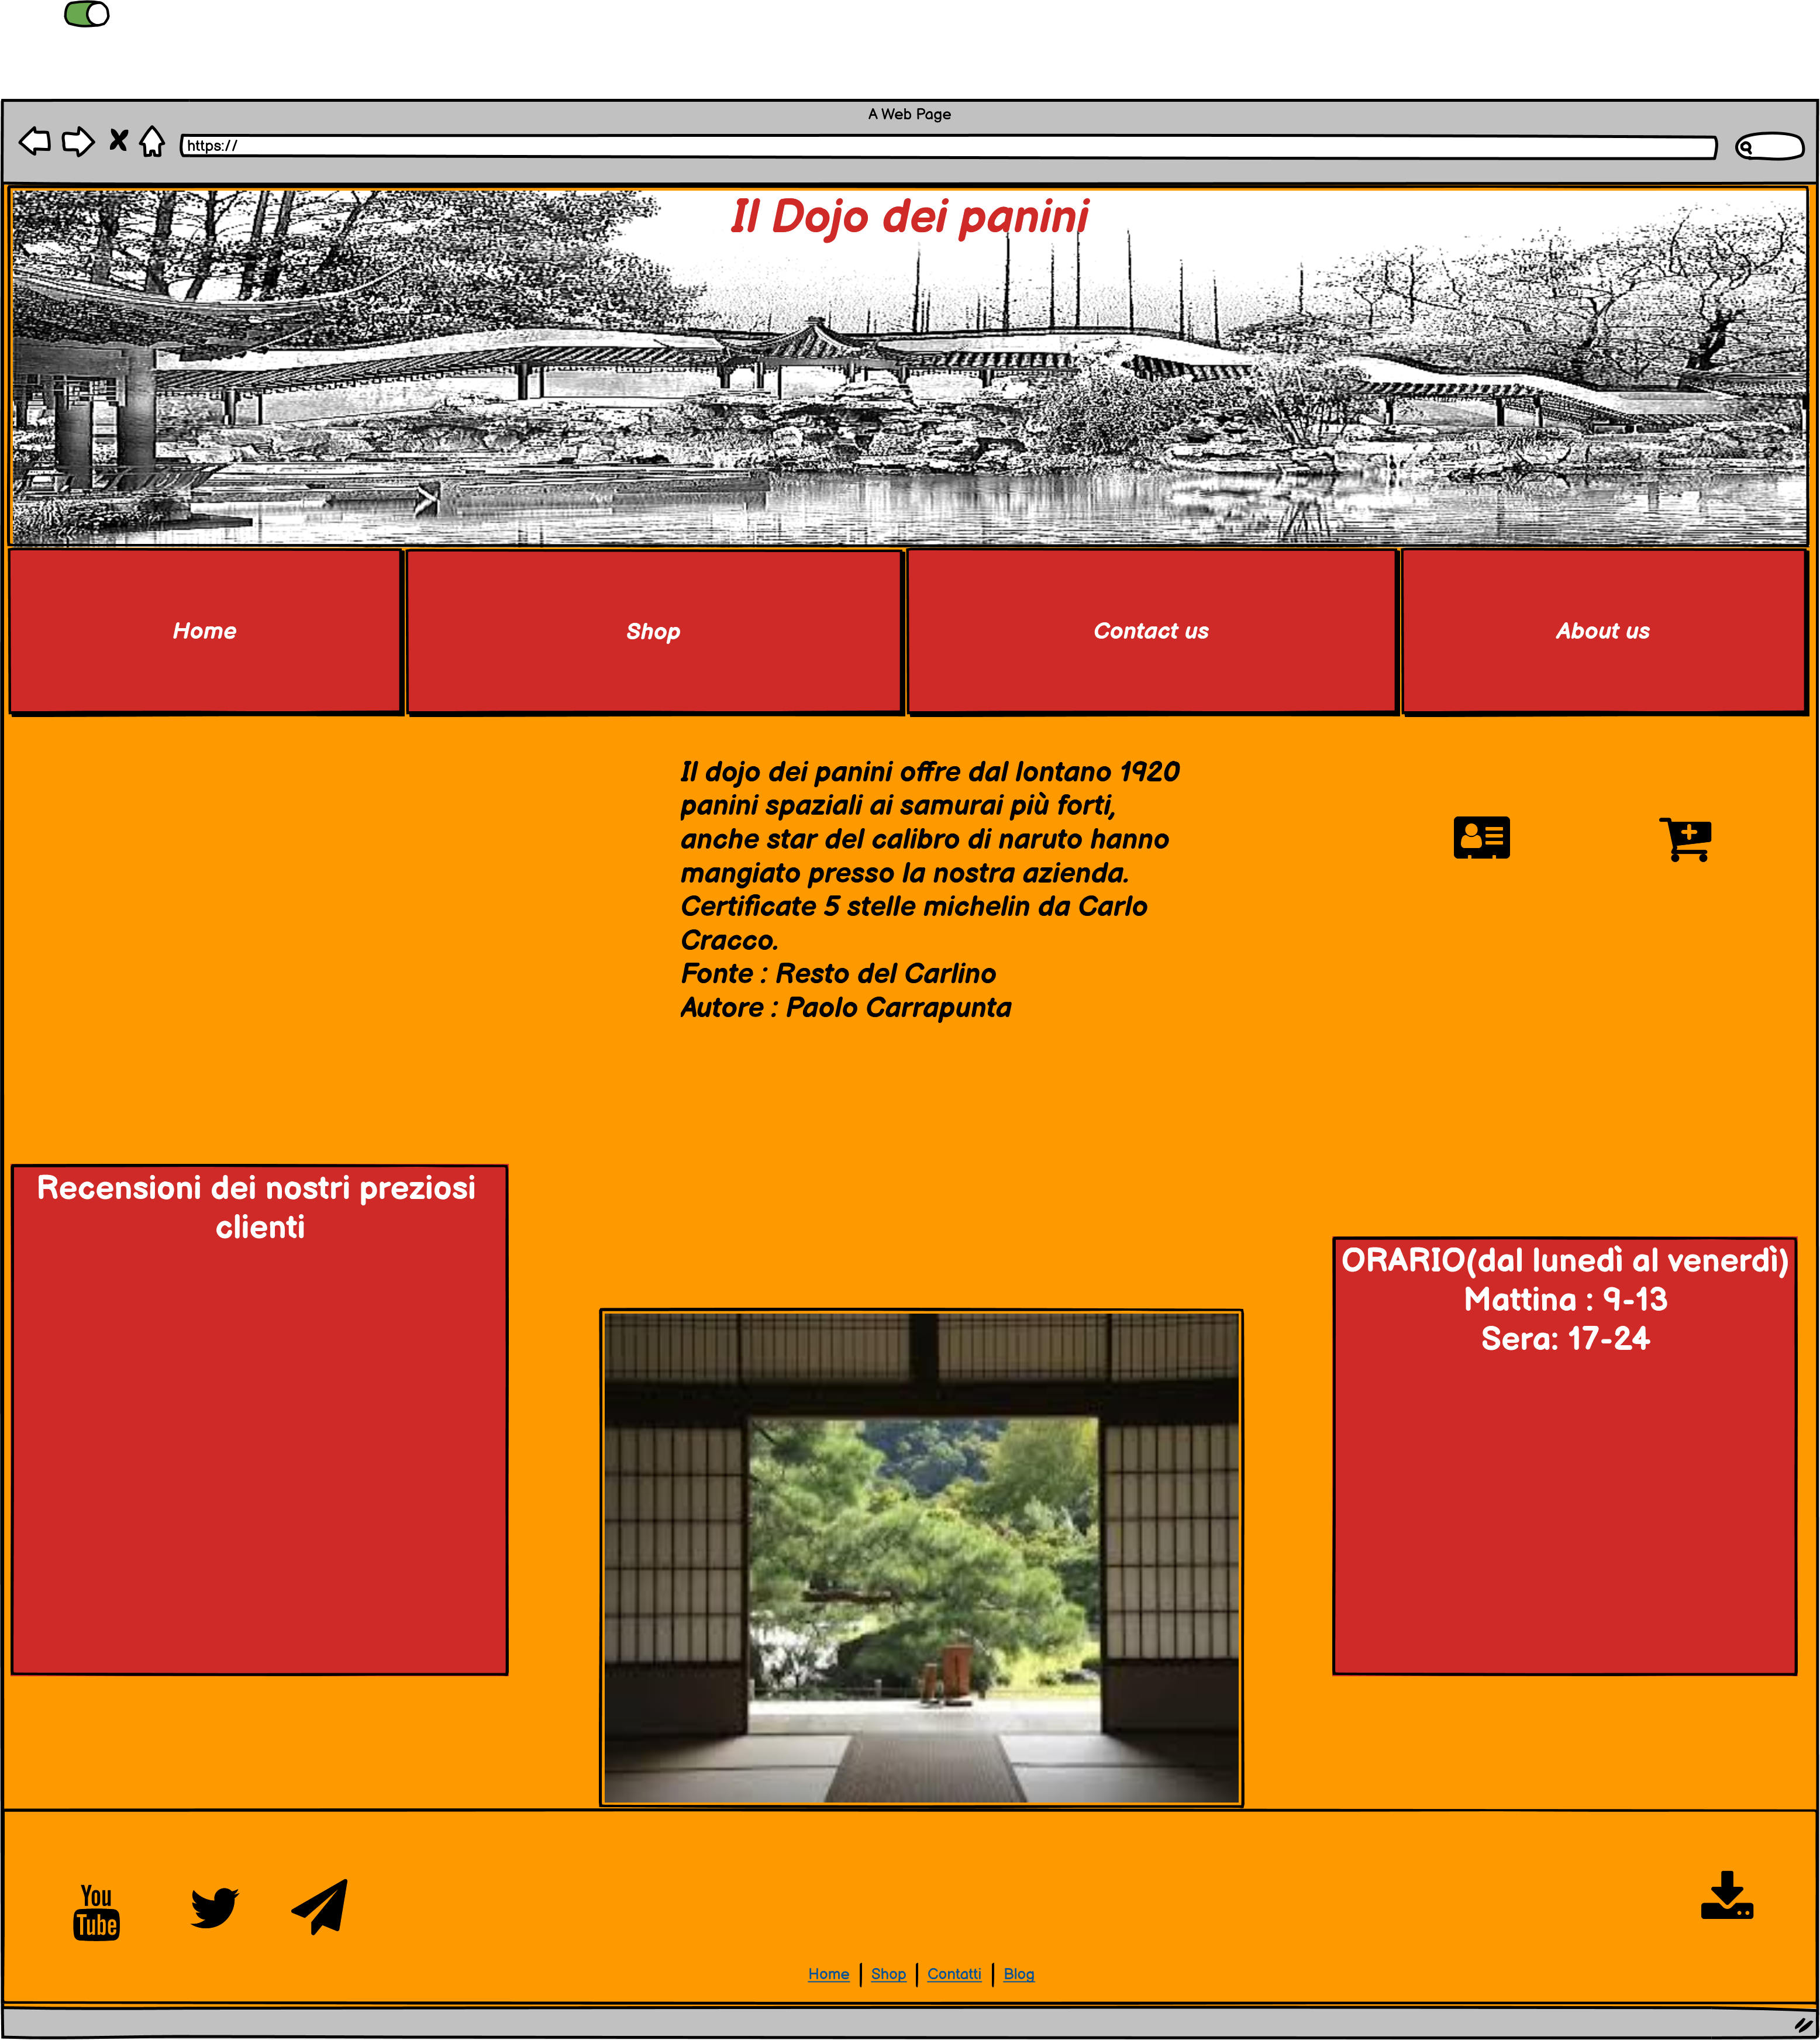
\includegraphics[width=1.2\textwidth, height=1.2\textheight, keepaspectratio]{./Images/Homepage.png}
		\caption{Homepage}
		\label{fig:homepage}
	\end{figure}

	% ======================== HOMEPAGE ==============================================
	
	\newpage
	
	%\enlargethispage{1\linewidth}
	
	\section{Homepage}
	
	\textsf{\small Questa è la pagina principale del sito, disponibile sia col tema chiaro che scuro. Da qui si può raggiungere tutte le altre pagine del sito quali: Shop, Login, Signup, About, Contatti, Menù.}\\
	
	\begin{figure}[ht] 
		\centering
		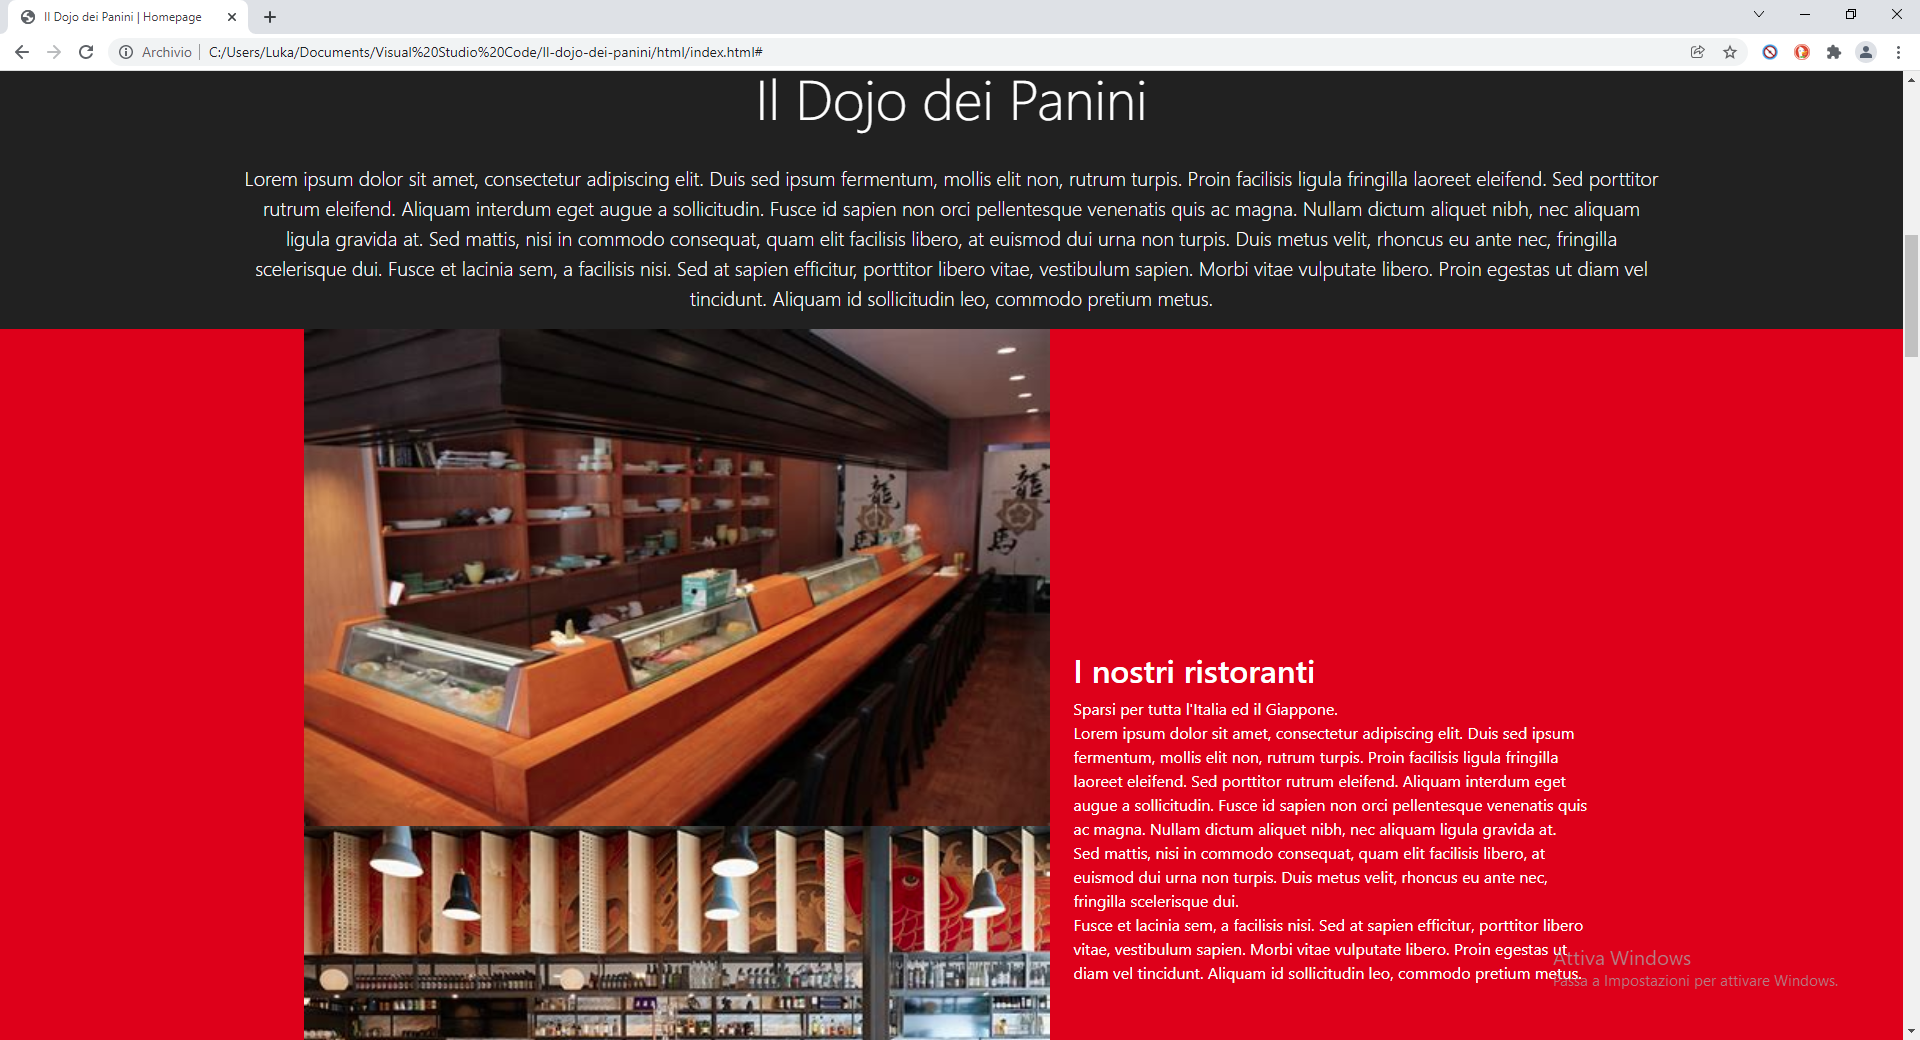
\includegraphics[width=1\textwidth, height=1\textheight, keepaspectratio]{./Images/Homepage_presentazione.png}
		\caption{Homepage sezione presentazione}
		\label{fig:homepage_presentazione}
	\end{figure}
	
	\textsf{\small L'homepage presenta: }
	
	\begin{itemize}
		\item \textsf{\small Una barra di navigazione}
		\item \textsf{\small Sezione di presentazione}
		\item \textsf{\small Alcuni panini del ristorante che potranno essere approfonditi nello shop o nel menù}
		\item \textsf{\small Una sezione delle recensioni del ristorante.}
		\item \textsf{\small Una sezione con una cartina geografica per indicare le varie località del ristorante.}
		\item \textsf{\small Un footer}
	\end{itemize}

	\begin{figure}[H] 
		\centering
		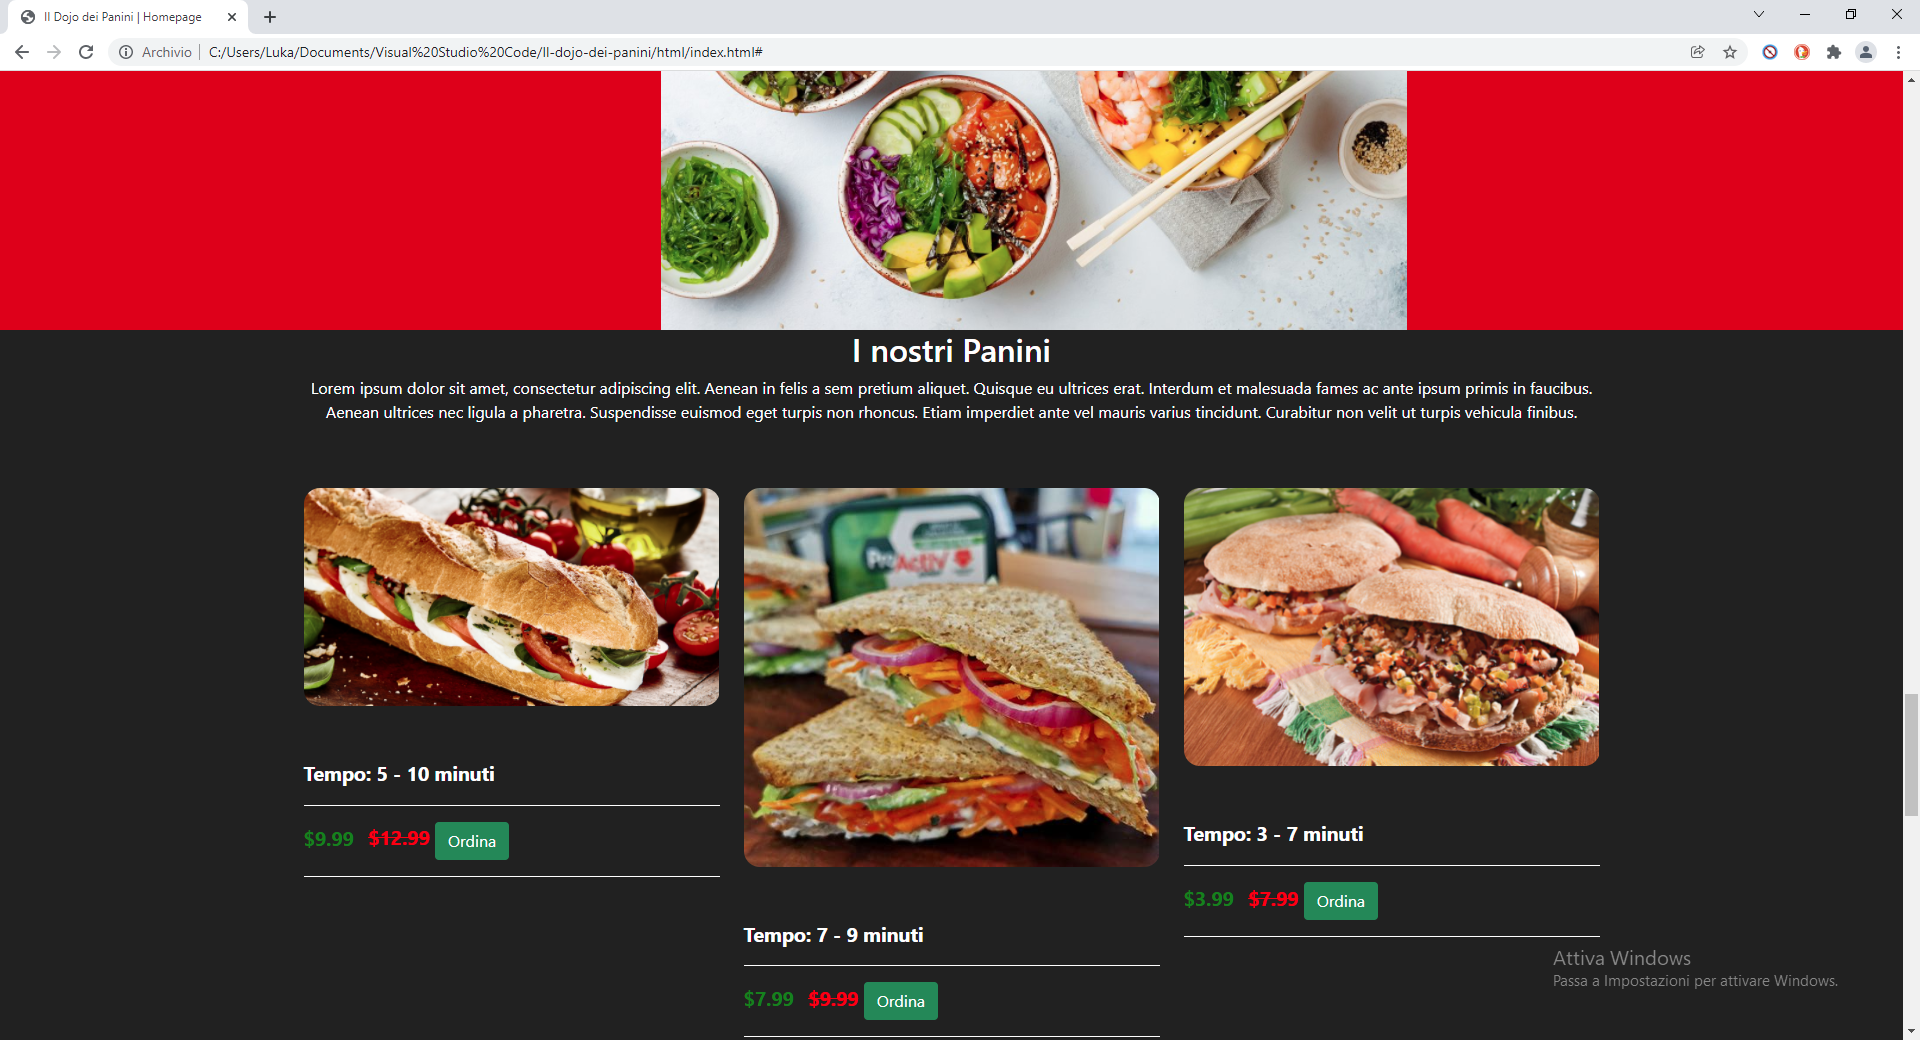
\includegraphics[width=1\textwidth, height=1\textheight, keepaspectratio]{./Images/Homepage_food.png}
		\caption{Homepage sezione cibo}
		\label{fig:homepage_cibo}
	\end{figure}

	\begin{figure}[H]
		\begin{subfigure}{.6\textwidth}
			\centering
			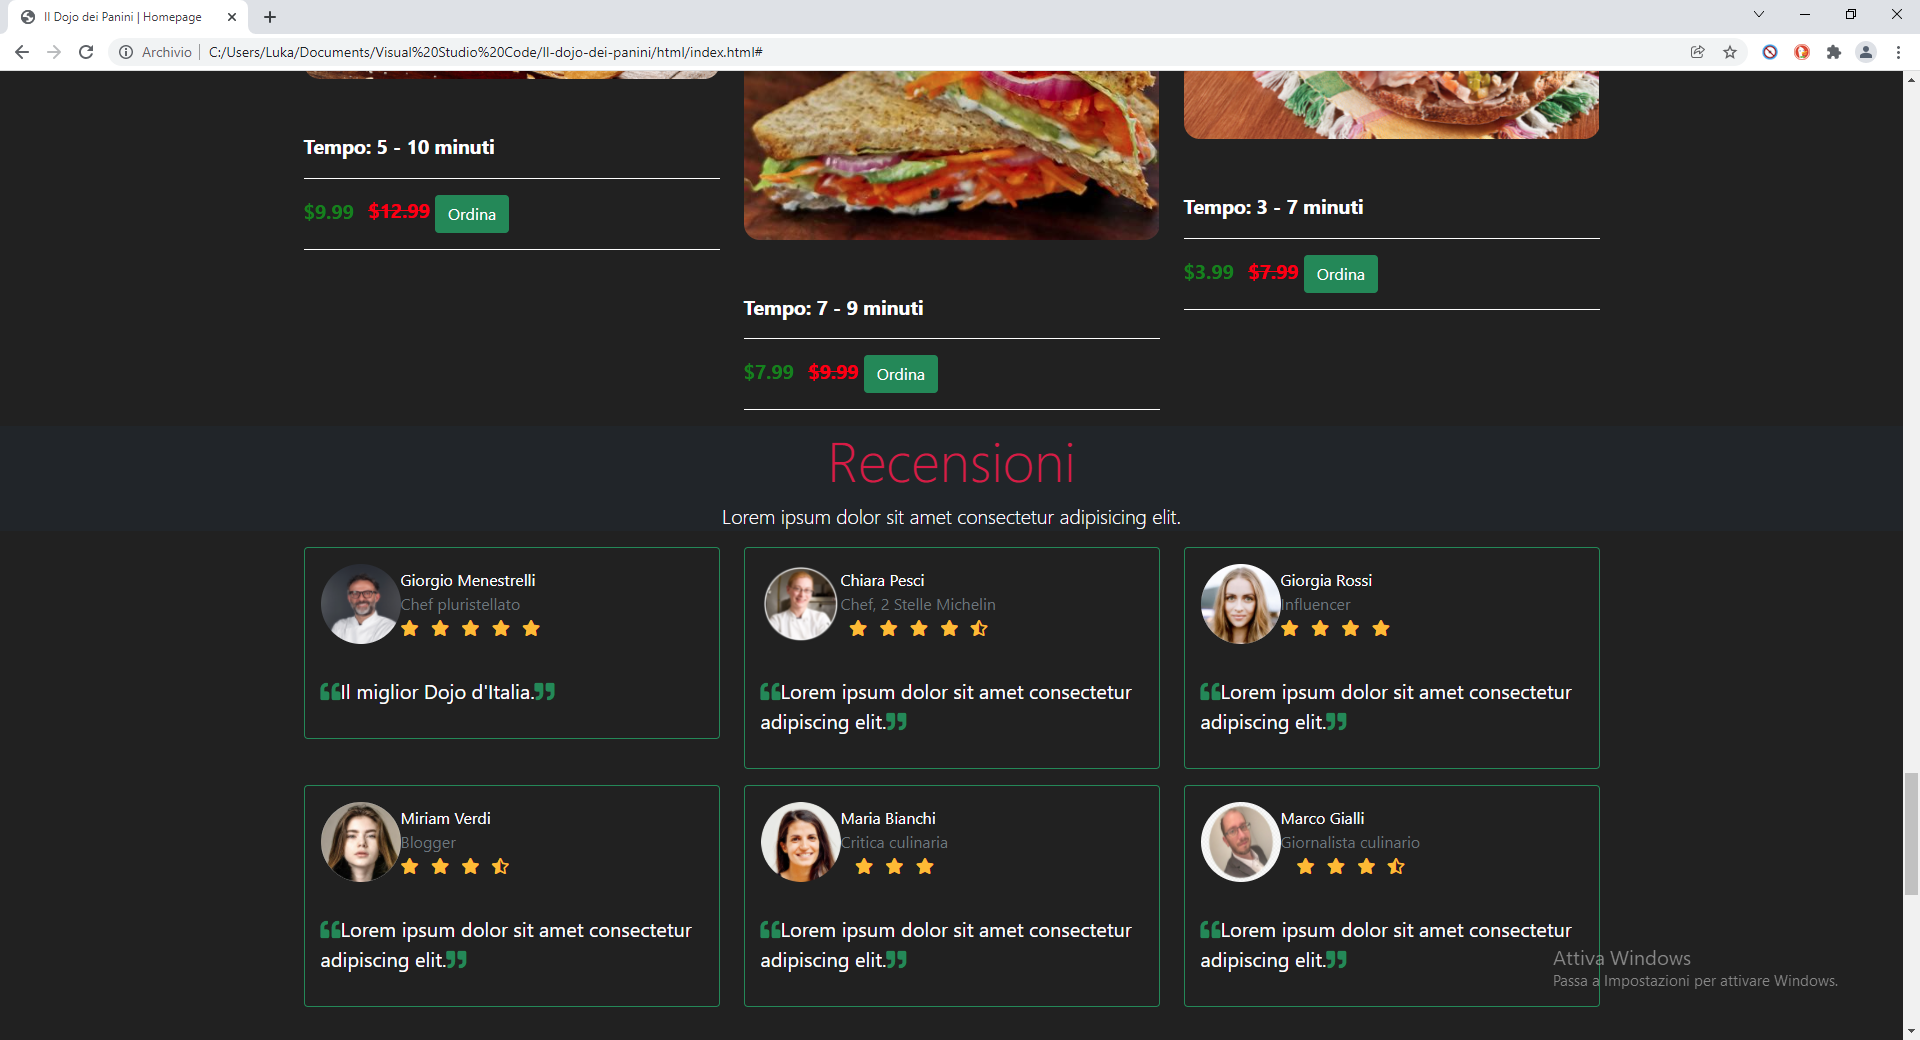
\includegraphics[width=1\linewidth]{./Images/Homepage_recensioni.png}
			\caption{Sezione delle recensioni}
			\label{fig:homepage_recensioni}
		\end{subfigure}
		\begin{subfigure}{.6\textwidth}
			\centering
			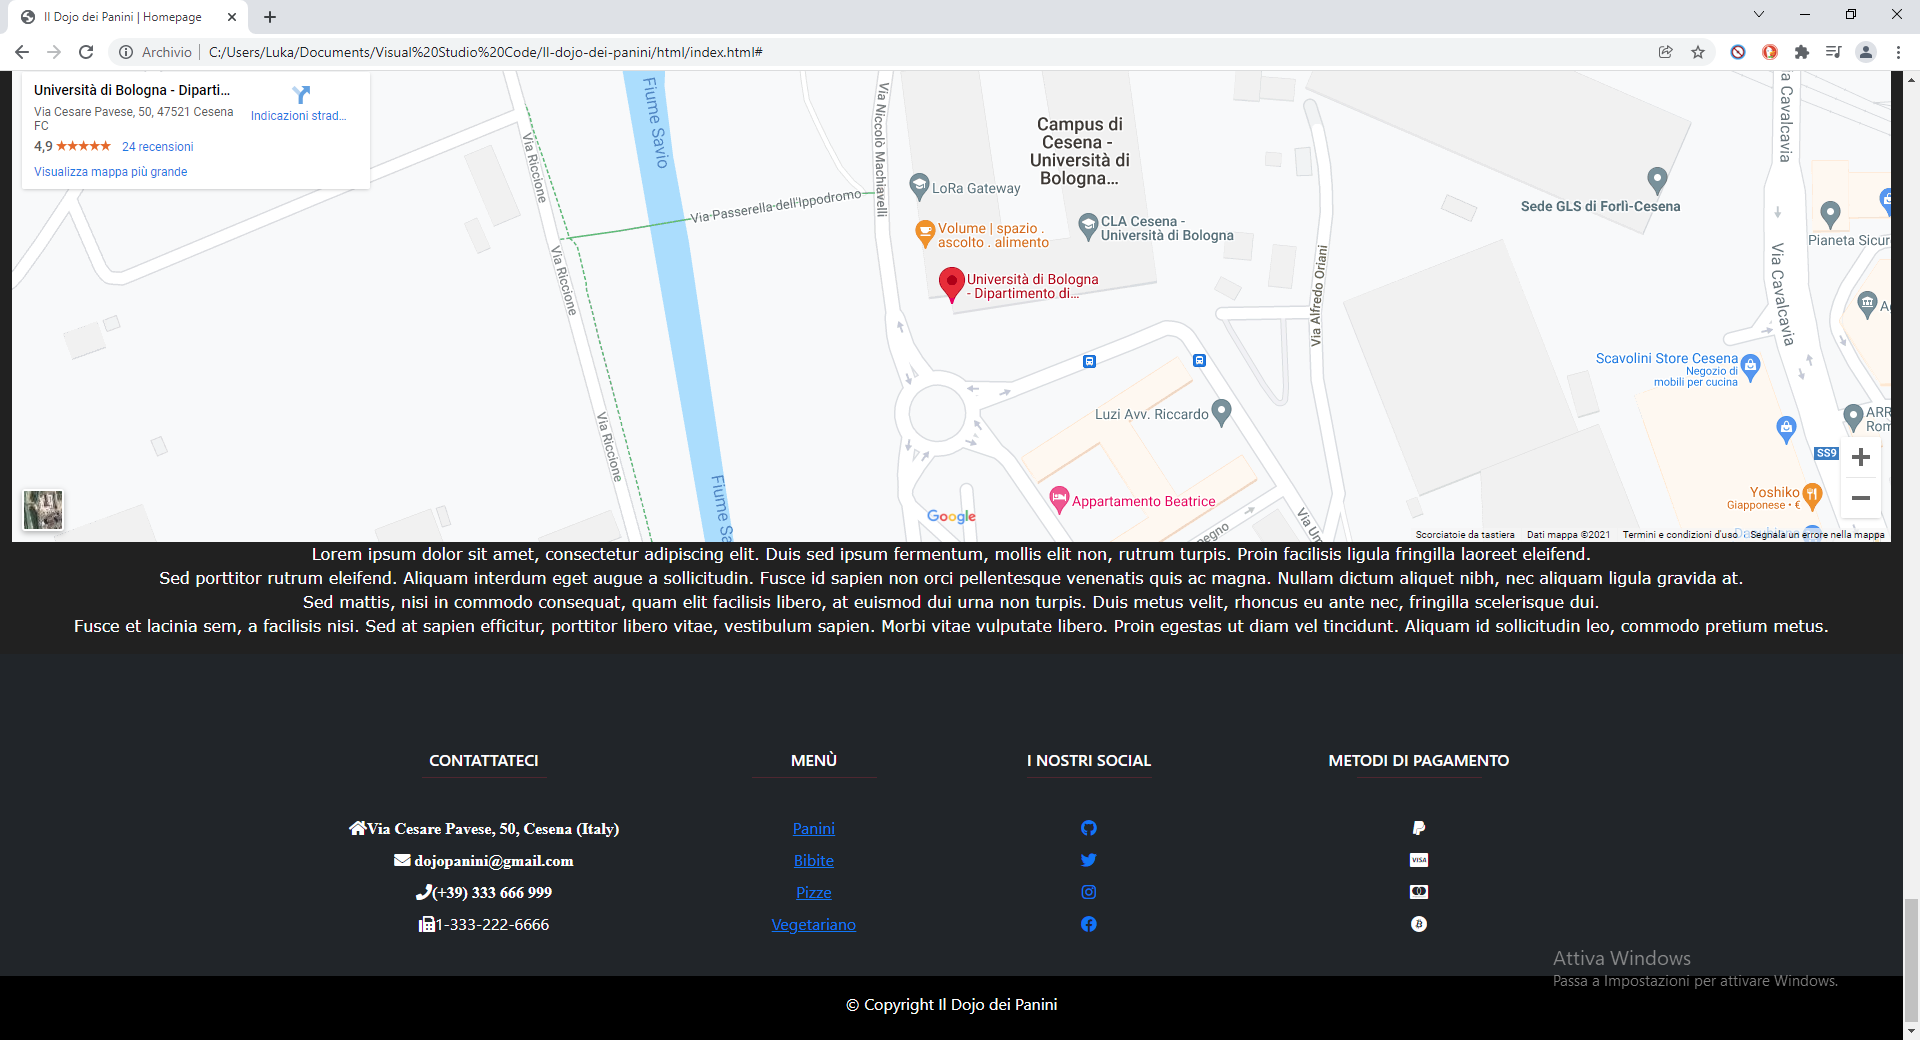
\includegraphics[width=1\linewidth]{./Images/Homepage_cartina_e_footer.png}
			\caption{Sezione cartina e footer}
			\label{fig:homepage_footer}
		\end{subfigure}
		%\caption{a}
		\label{fig:homepages}
	\end{figure}

	% ======================== LOGIN E SIGNUP ========================================
	
	\newpage
	
	\section{Login | Signup | Forgot password}
	
	\textsf{\small L'utente e l'admin possono collegarsi al loro account attraverso la pagina di \emph{login}.}
	\textsf{\small Per poter entrare l'utente può sia utilizzare la sua email sia il suo username.}\\
	\textsf{\small L'admin invece può entrare solo con lo username e il suo username deve iniziare con la keyword \emph{admin}.}\\
	\textsf{\small Se l'utente non ha un account può crearne uno dalla pagina di \emph{signup}.}
	
	\begin{figure}[H] 
		\centering
		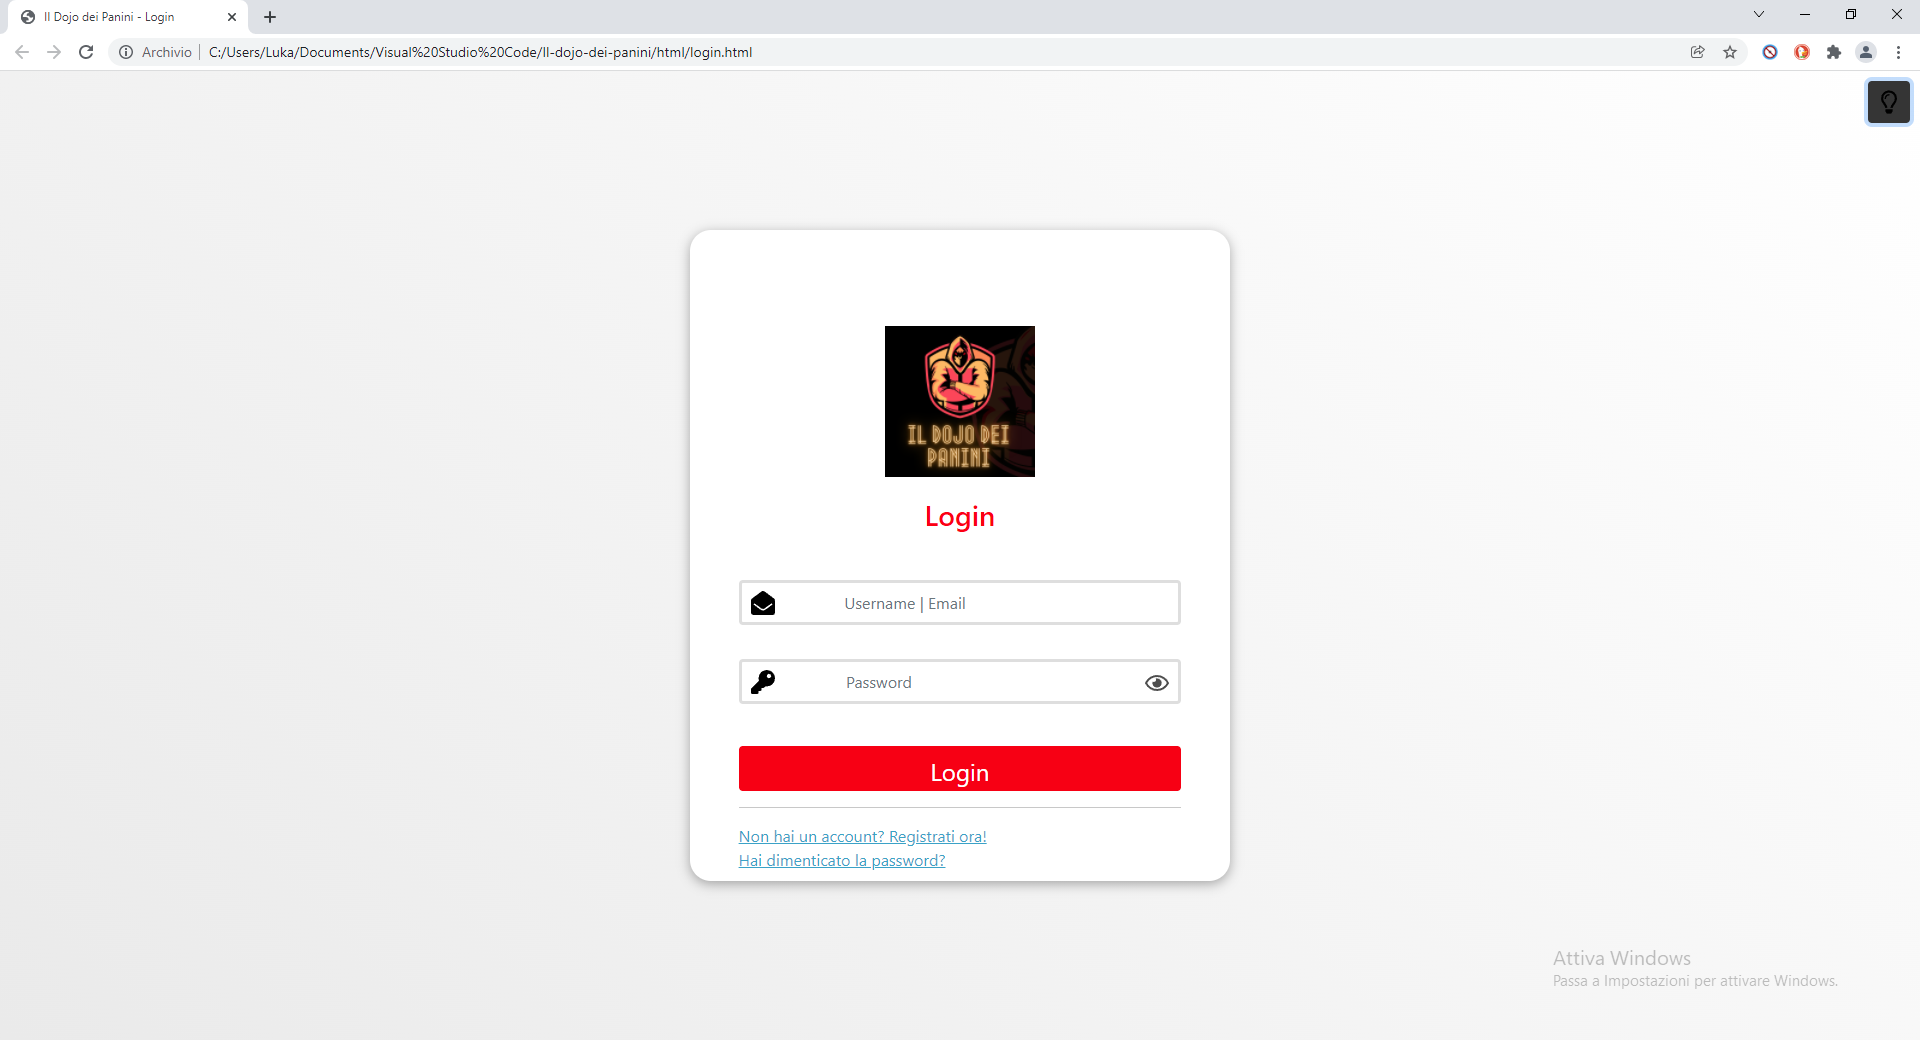
\includegraphics[width=1\textwidth, height=1\textheight, keepaspectratio]{./Images/Login.png}
		\caption{Pagina di Login}
		\label{fig:login}
	\end{figure}
	
	\begin{figure}[H]
		\begin{subfigure}{.6\textwidth}
			\centering
			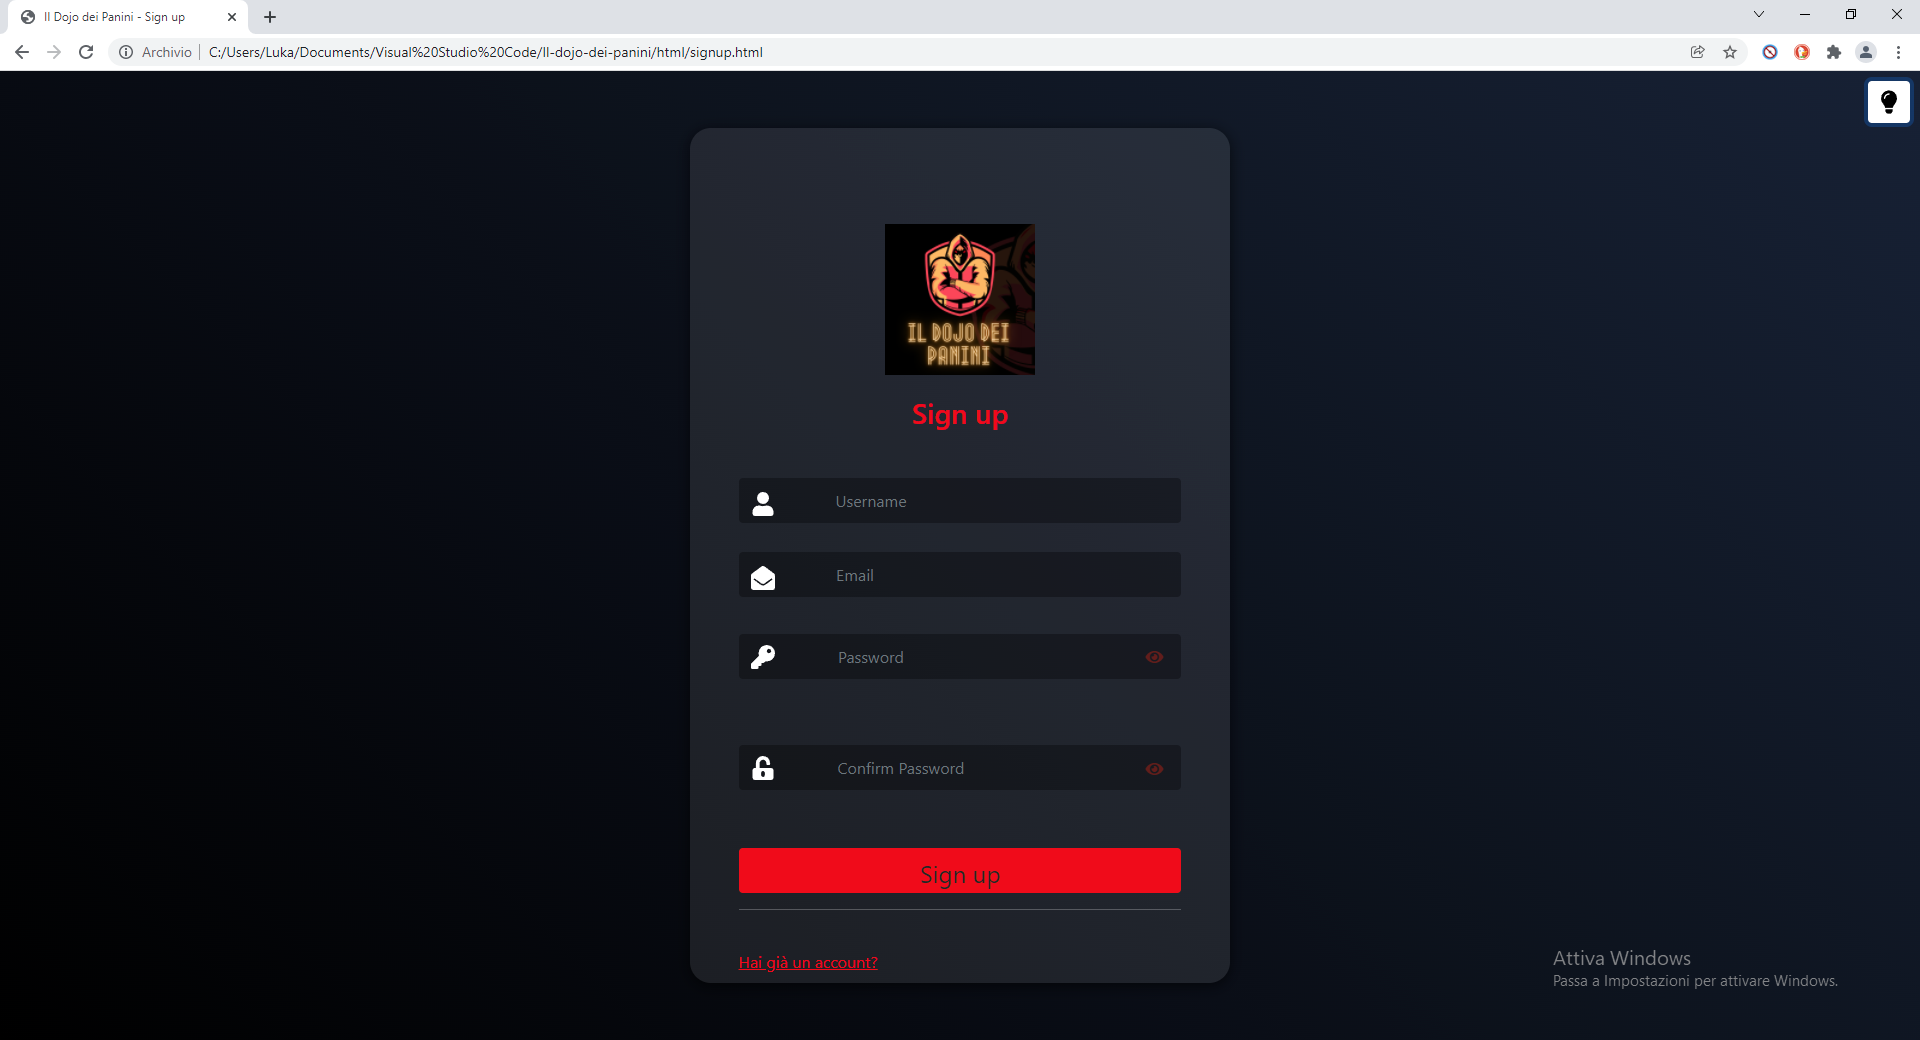
\includegraphics[width=1\linewidth]{./Images/Signup.png}
			\caption{Pagina di signup}
			\label{fig:signup}
		\end{subfigure}
		\begin{subfigure}{.6\textwidth}
			\centering
			%TODO: 
			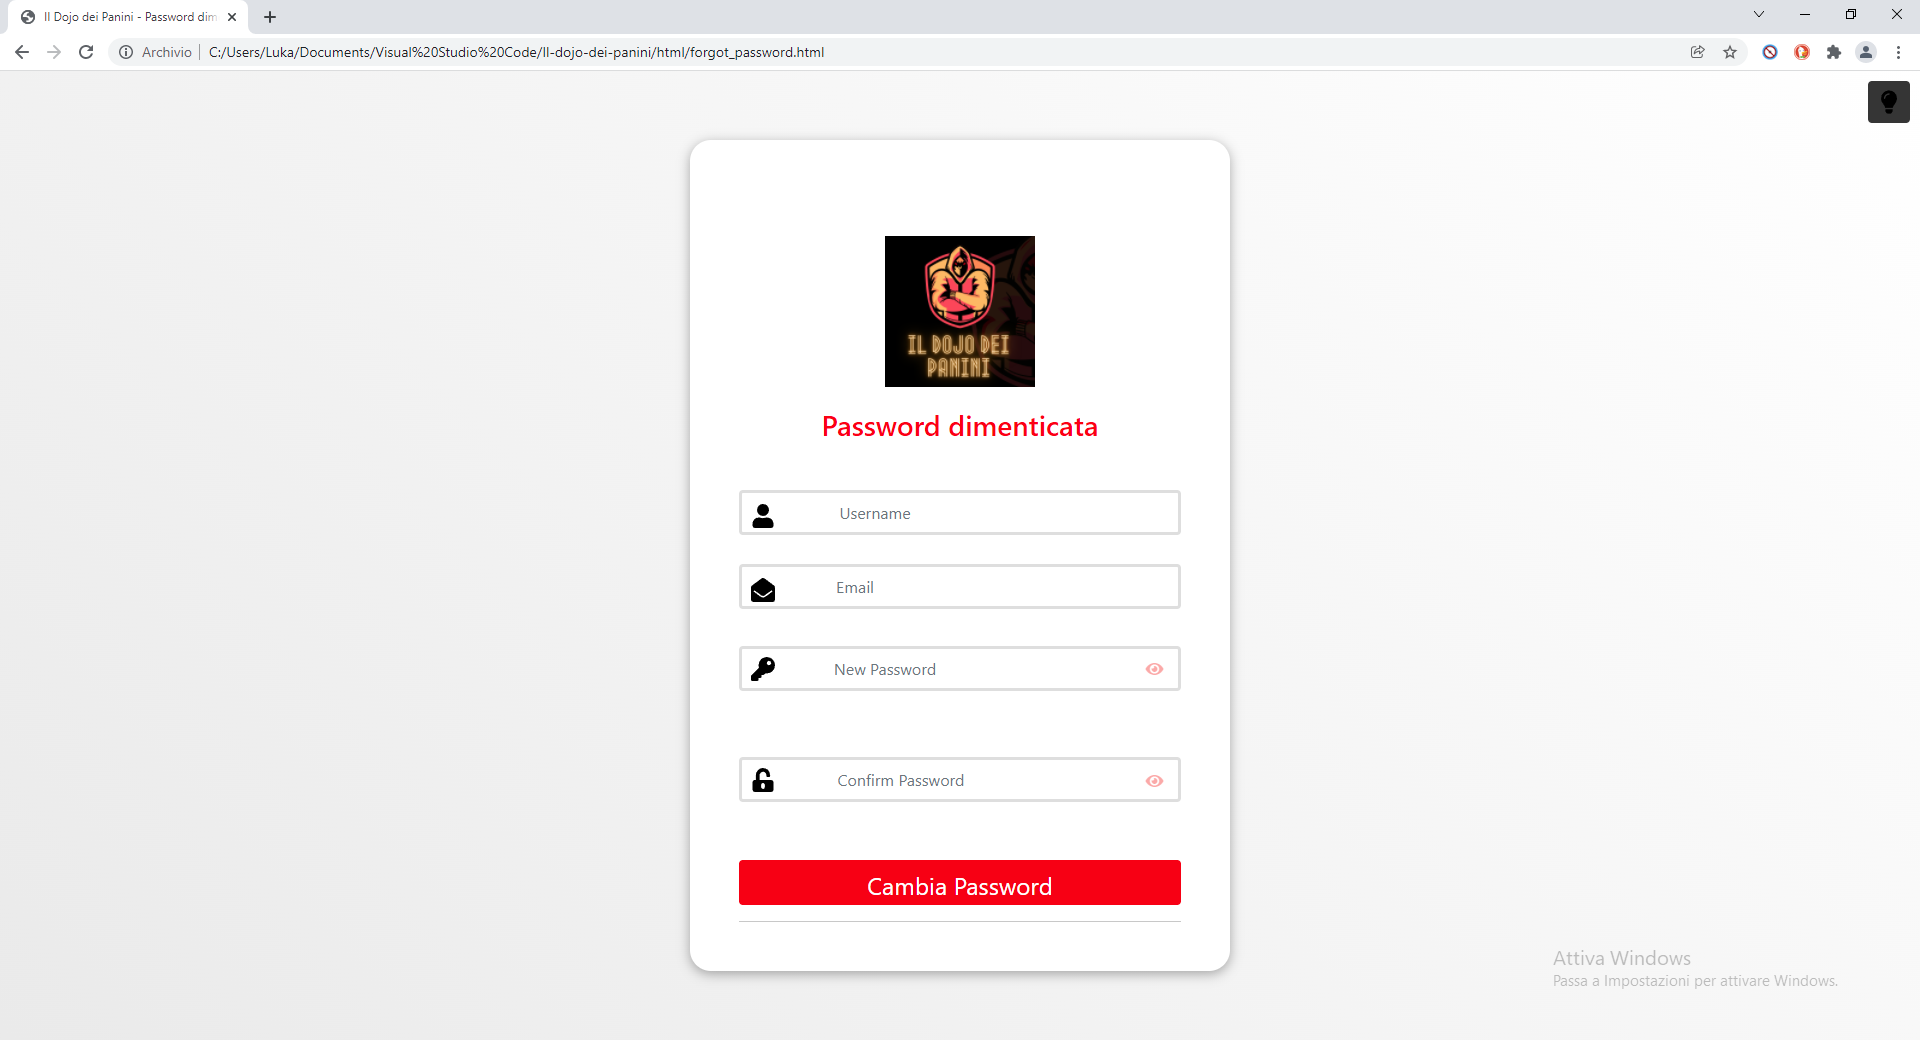
\includegraphics[width=1\linewidth]{./Images/Forgot_password.png}
			\caption{Pagina per recuperare la password}
			\label{fig:forgot-password}
		\end{subfigure}
		%\caption{a}
		\label{fig:}
	\end{figure}

	\textsf{\small Inoltre, l'utente può recuperare la sua password se se l'è scordata attraverso la pagina \emph{forgot\_password}.}
	\textsf{\small Tutte queste pagine presentano una versione col tema scuro e una con il tema chiaro.}\\
	
	\textsf{\small Inoltre, la pagina di signup ha un controllo sulla forza della password e un controllo se la password inserita nell'input primario e di conferma combaciano.}\\
	\textsf{\small Inoltre, tutte queste pagine condividono la funzionalità di poter far comparire e scomparire la password inserita cliccando l'icona dell'occhio.}\\
	
	% ======================== LOGIN SEZIONE UTENTE ==================================
	
	\newpage
	
	\section{Login sezione Utente}
	
	\textsf{\small Una volta loggato, l'utente avrà la possibilità di aggiungere prodotti al carrello, di rimuoverne e di comprarli passando alla sezione acquisti.}\\
	
	%TODO: Modificare la sezione shop e aggiungere l'immagine/i
	
	\subsection{Shop}
	
	\textsf{\small Attraverso la pagina dello \emph{Shop}, l'utente potrà aggiungere i prodotti al suo carrello personale.}\\
	
	\begin{figure}[H] 
		\centering
		%TODO: uncomment \includegraphics qua sotto ed inserire l'immagine
		%\includegraphics[width=1\textwidth, height=1\textheight, keepaspectratio]{./Images/}
		\caption{Pagina dello Shop}
		\label{fig:shop}
	\end{figure}
	
	%TODO: Modificare la sezione carrello e aggiungere l'immagine/i
	
	\subsection{Carrello}
	
	\textsf{\small Mediante la pagine del \emph{carrello} è possibile modificare gli ordini, aumentandone o diminuendone la quantità di prodotti.}\\
	
	\begin{figure}[H] 
		\centering
		%TODO: uncomment \includegraphics qua sotto ed inserire l'immagine
		%\includegraphics[width=1\textwidth, height=1\textheight, keepaspectratio]{./Images/}
		\caption{Pagina del Carrello}
		\label{fig:carrello}
	\end{figure}
	
	%TODO: Messaggi e notifiche e aggiungere l'immagine/i
	
	\subsection{Messaggi}
	
	\textsf{\small Grazie alla pagine dei messaggi l'utente può visionare i messaggi ricevuti dal sito, quali: Notifiche di Login, ordini eseguiti, ecc..}\\
	
	\begin{figure}[H] 
		\centering
		%TODO: uncomment \includegraphics qua sotto ed inserire l'immagine
		%\includegraphics[width=1\textwidth, height=1\textheight, keepaspectratio]{./Images/}
		\caption{Pagina dei Messaggi}
		\label{fig:messaggi}
	\end{figure}
	
	% ======================== LOGIN SEZIONE ADMIN ===================================
	
	\newpage
	
	\section{Login sezione Admin}
	
	\textsf{\small Una volta loggato, l'admin avrà accesso a tutti i prodotti presenti e potrà inoltre aggiungerne, modificarne e rimuoverne.}\\
	
	\begin{figure}[H] 
		\centering
		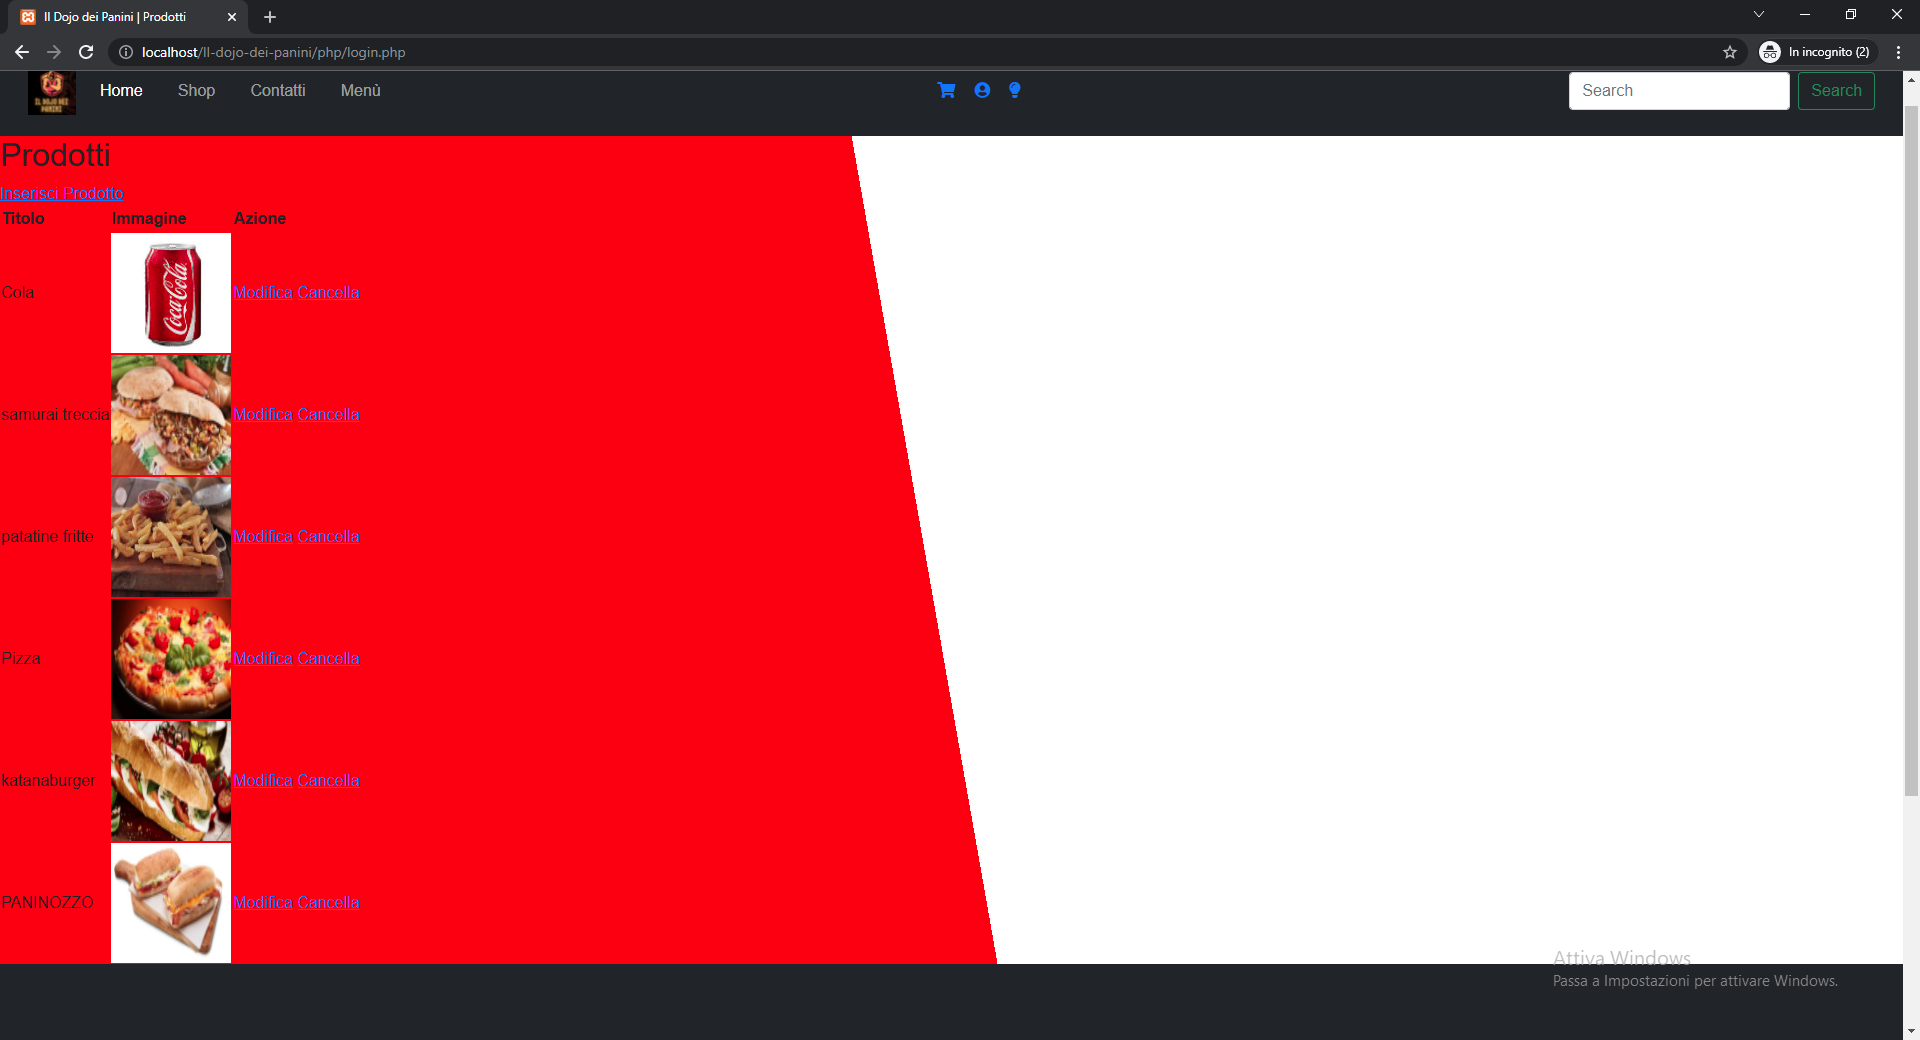
\includegraphics[width=1\textwidth, height=1\textheight, keepaspectratio]{./Images/Admin.png}
		\caption{Pagina dell'Admin}
		\label{fig:admin}
	\end{figure}

	\begin{figure}[H]
		\begin{subfigure}{.6\textwidth}
			\centering
			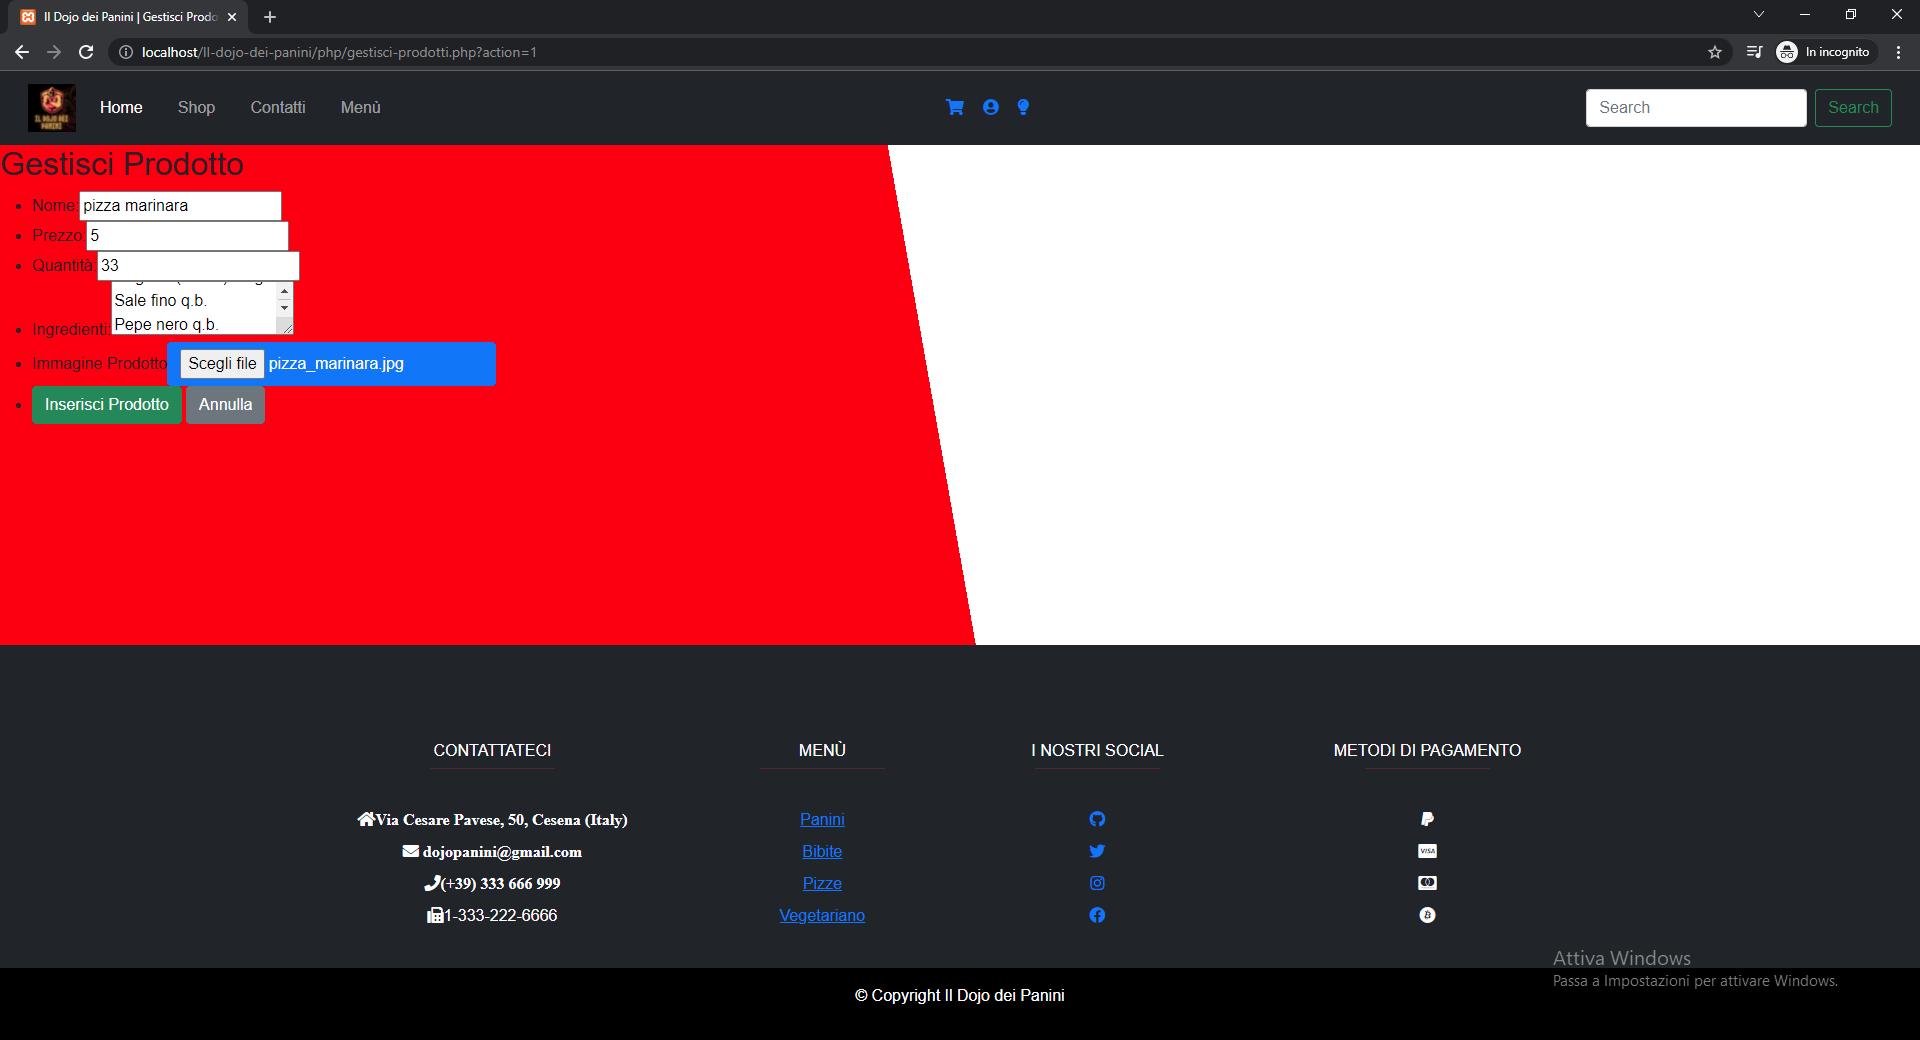
\includegraphics[width=1\linewidth]{./Images/Admin_inserimento.png}
			\caption{Pagina di inserimento del prodotto}
			\label{fig:inserimento1}
		\end{subfigure}
		\begin{subfigure}{.6\textwidth}
			\centering
			%TODO: 
			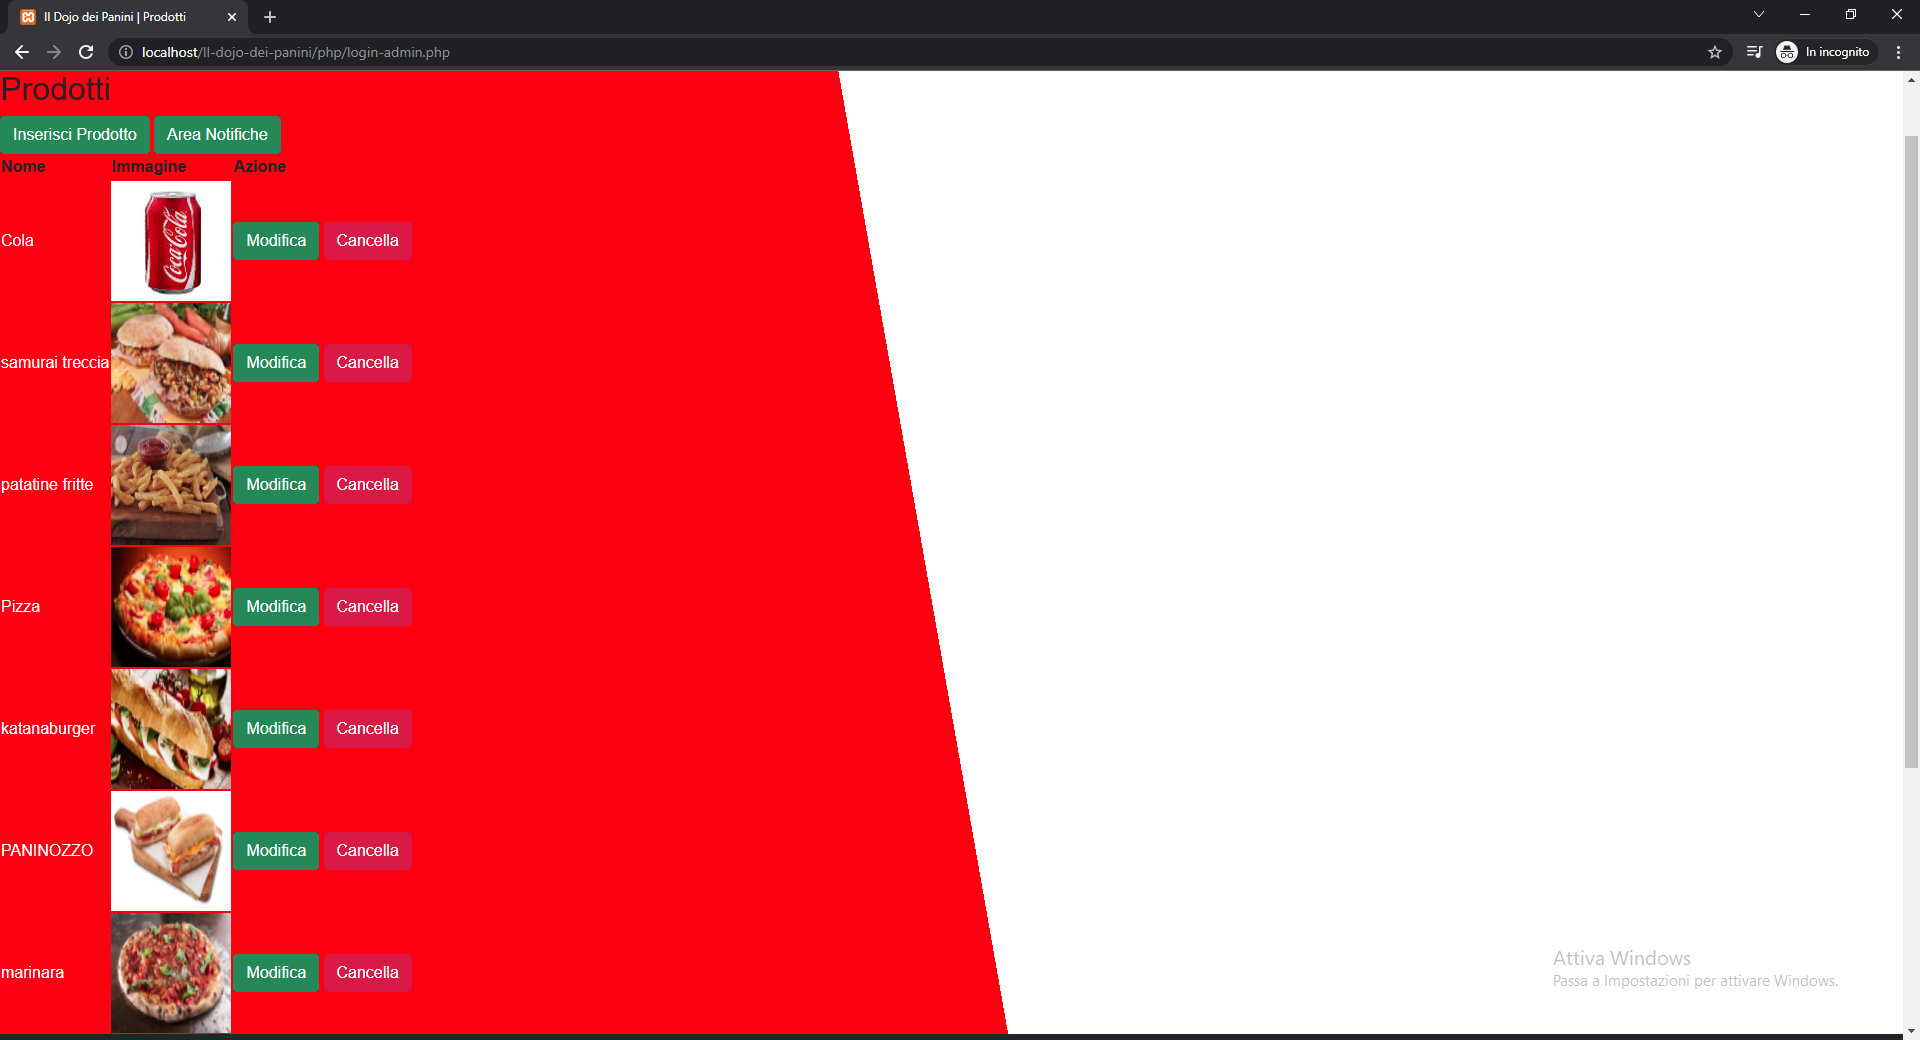
\includegraphics[width=1\linewidth]{./Images/Admin_inserimento2.png}
			\caption{Prodotto inserito in lista}
			\label{fig:inserimento2}
		\end{subfigure}
		%\caption{a}
		\label{fig:inserimenti}
	\end{figure}

	\begin{figure}[H]
		\begin{subfigure}{.6\textwidth}
			\centering
			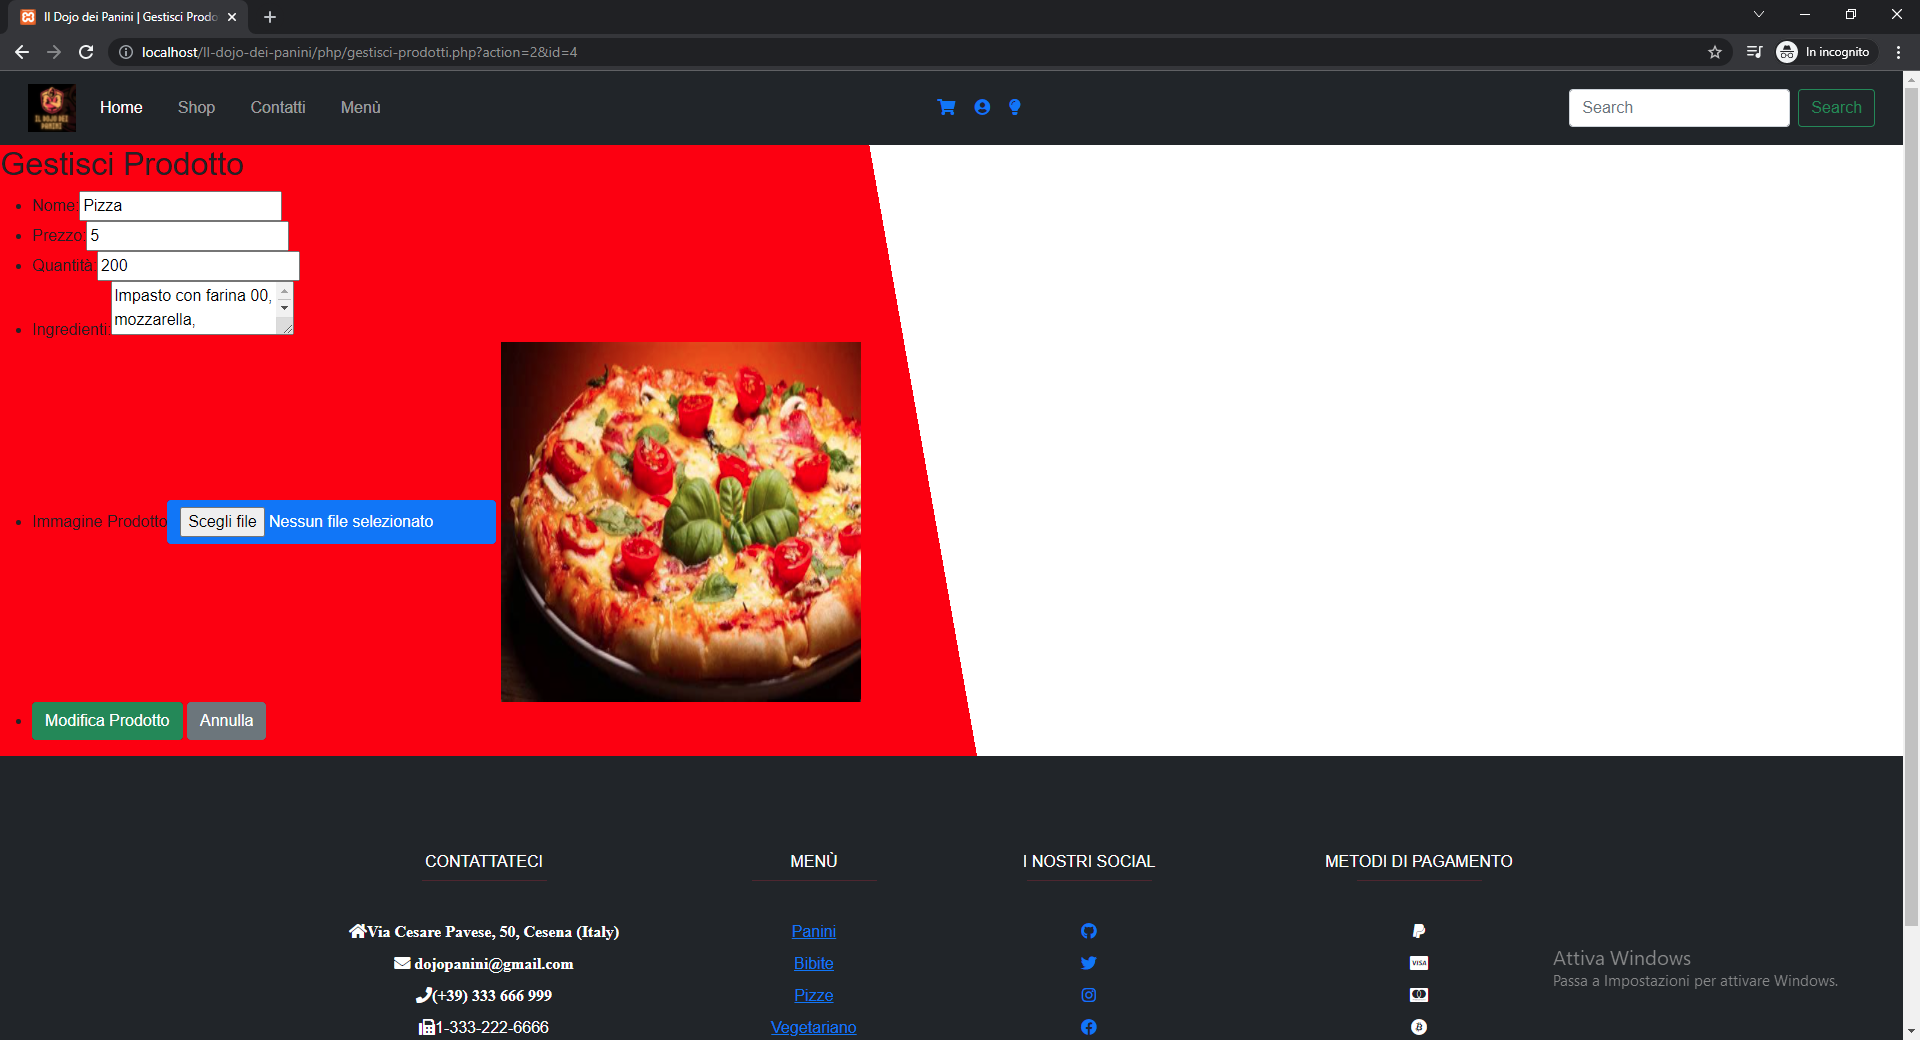
\includegraphics[width=1\linewidth]{./Images/Admin_modifica_prodotto.png}
			\caption{Pagina di modifica del prodotto}
			\label{fig:modifica}
		\end{subfigure}
		\begin{subfigure}{.6\textwidth}
			\centering
			%TODO: 
			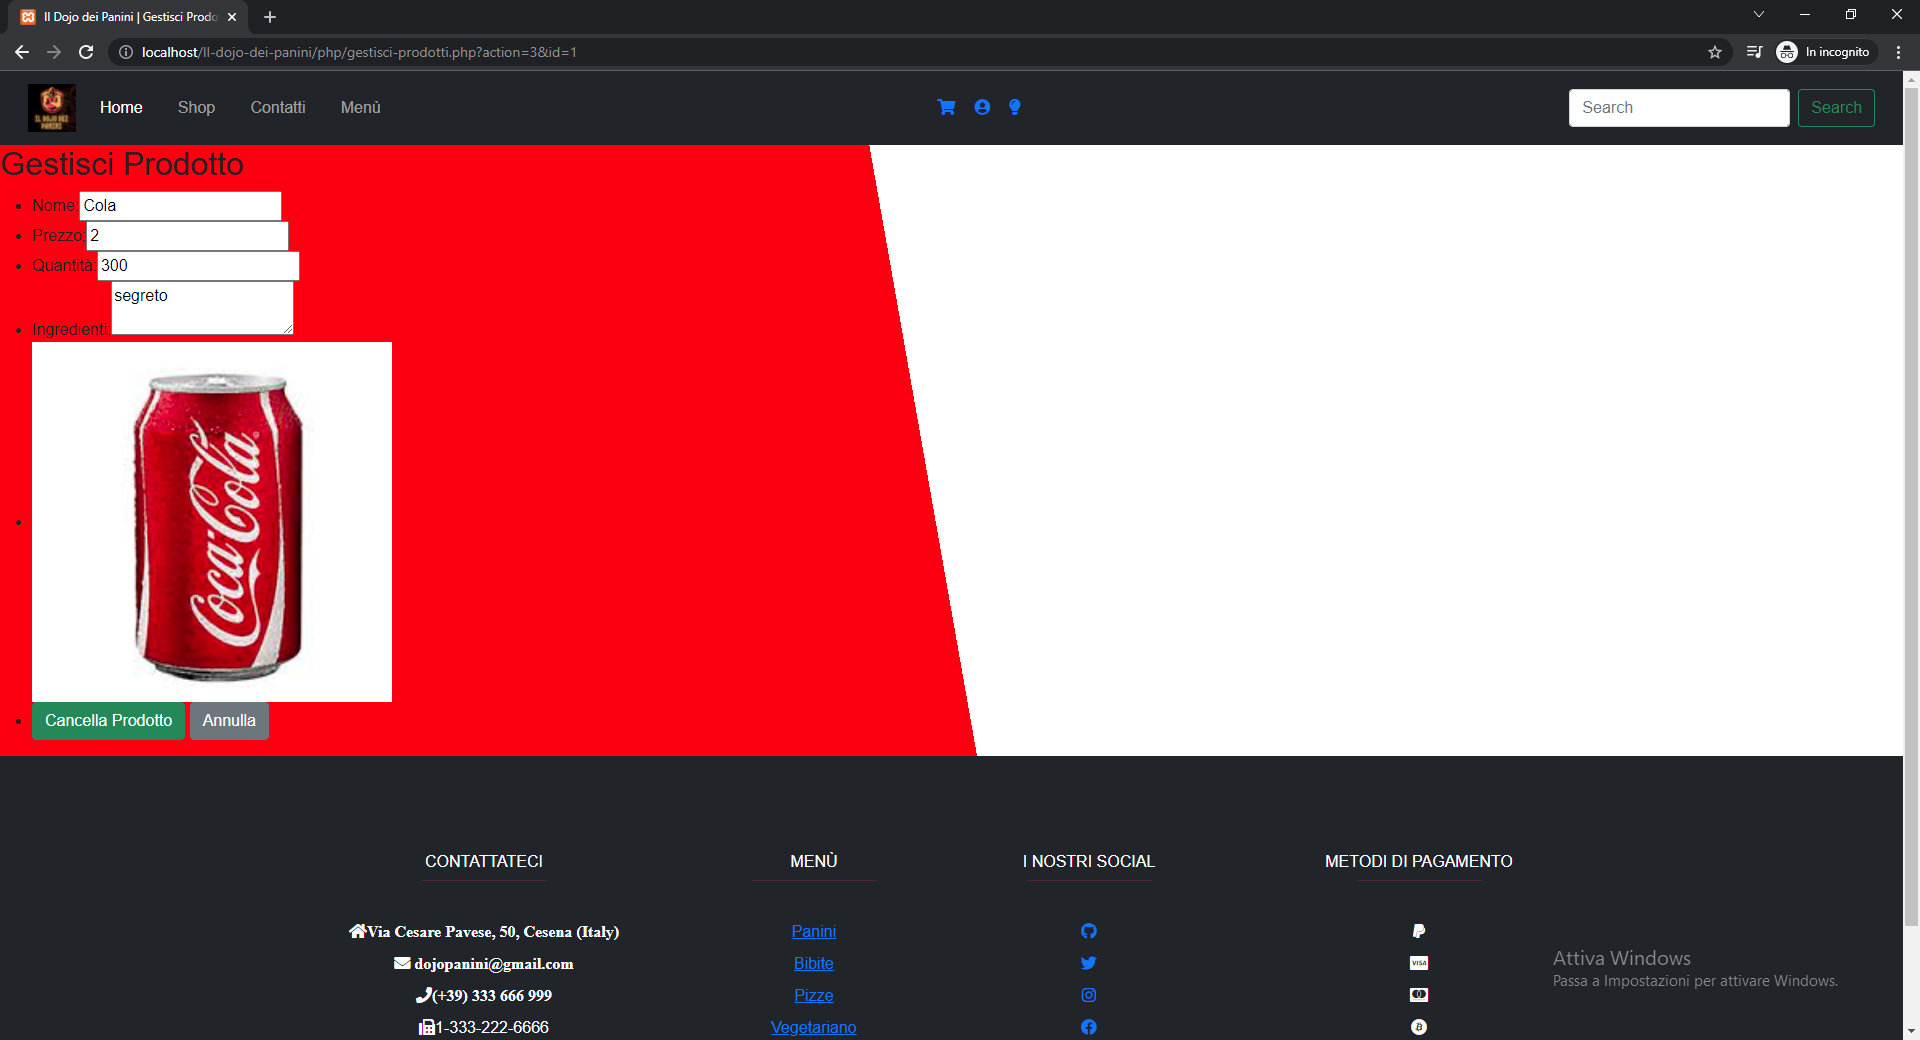
\includegraphics[width=1\linewidth]{./Images/Admin_cancella_prodotto.png}
			\caption{Prodotto cancellato dalla lista}
			\label{fig:cancella}
		\end{subfigure}
		%\caption{a}
		\label{fig:operazioni_sul_prodotto}
	\end{figure}

	\textsf{Una volta aggiunto, modificato o cancellato un prodotto, l'admin riceverà una notifica nella sua sezione \emph{Area Notifiche}.}\\
	
	\begin{figure}[H] 
		\centering
		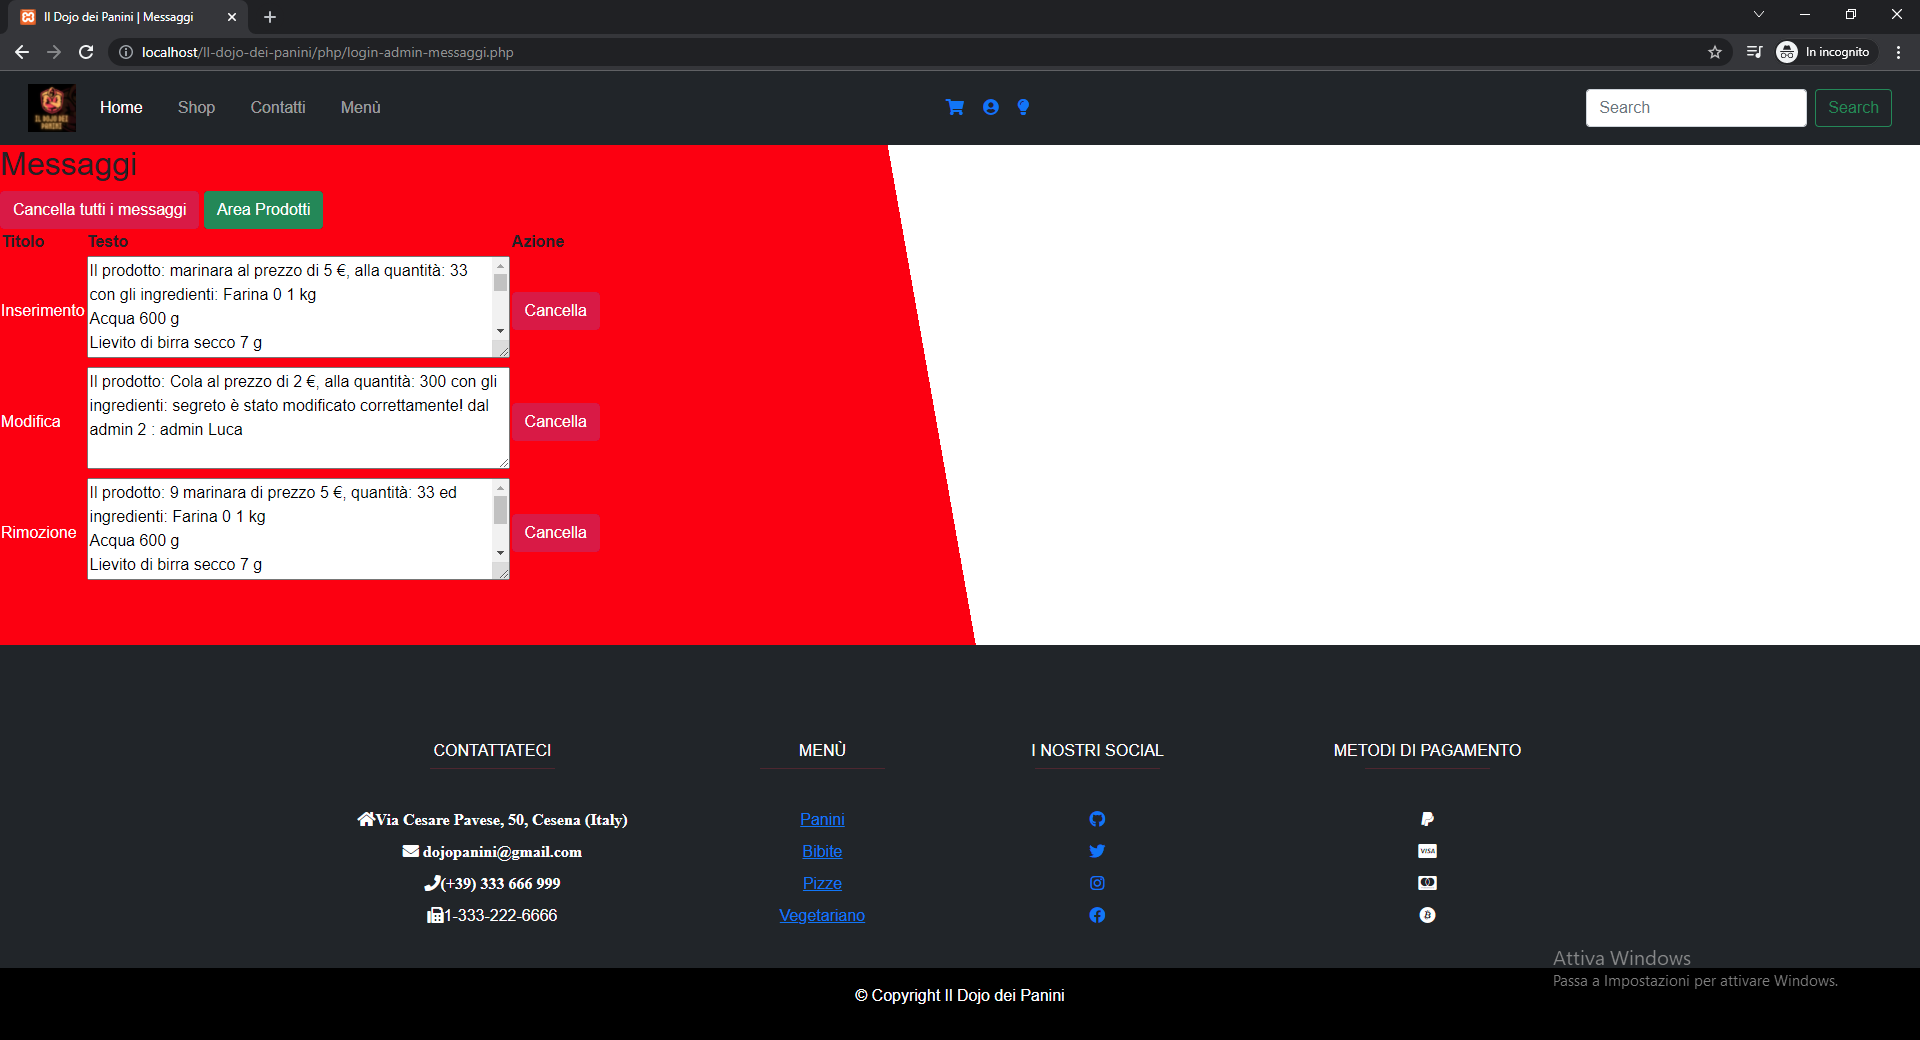
\includegraphics[width=1.2\textwidth, height=1.2\textheight, keepaspectratio]{./Images/Admin_area_notifiche.png}
		\caption{Area Notifiche}
		\label{fig:notifiche}
	\end{figure}
	
	% ======================== DOMINIO APPLICATIVO ===================================
	%TODO: decidere se questa parte la vogliamo tenere o modificare, ecc..
	
	\newpage
	
	\section{Dominio applicativo}
	Vendita di panini con consegna a domicilio in 8 minuti max, eco friendly(consegne in bici elettrica e tesla).
	
	\section{Tecnologie utilizzate}
	\begin{itemize}
		\item lato client : \textbf{HTML}
		\item stile : \textbf{BOOTSTRAP, CSS}
		\item lato server : \textbf{PHP}
	\end{itemize}

	\section{Applicativo}
	
	\subsection{Versione 1 - base(solo componenti obbligatorie)}
	\begin{itemize}
		\item login e pagina dedicata a venditore e cliente
		\item aggiungere prodotti lato venditore
		\item creare una lista di prodotti(paninozzi) acquistabili
		\item carrello e acquisto di prodotti selezionati da lista
		\item mostrare i prodotti nel carrello(tabella dinamica)
		\item mostrare lista dei prodotti, lato venditore(tabella dinamica)
		\item notifica per l'acquisto(successo o insuccesso)
		\item notifica per la vendita
		\item simulazione del pagamento
		\item in caso di portafogli vuoto warning
	\end{itemize}

	\subsection{Versione definitiva - con effetti wow}
	\begin{itemize}
		\item Utilizzo di ajax
		\item Accessibile per chi utilizza lo screen reader
		\item Aggiunta di recensioni 
	\end{itemize}

	\section{Software per Mockup utilizzati}
	
	\begin{itemize}
		\item Figma
		\item Balsamiq
	\end{itemize}

	% ================= GUIDA UTENTE =================================================
	%TODO: la guida utente è da tenere.
	
	\newpage

	\section{Guida utente}
	L'utente in prima istanza visualizzerà la homepage del sito, da lì avrà la possibilità di accedere.
	L'accesso potrà essere sia customer-side(cliente) e vendor-side(venditore).
	Dal lato customer-side potrà comprare e farsi spedire i prodotti, lasciare recensioni, visualizzare il catalogo, ecc. ecc.
	Dal lato vendor-side verranno gestite le liste di prodotti, ovviamente la vendita e tanto altro.\\
	
	\textsf{\small Qui, di seguito verranno indicate le procedure e le istruzioni da eseguire per poter avviare correttamente il sito web: } \\
	
	\begin{itemize}
		\item \textsf{\small Eseguire nella directory \emph{db} il file \emph{create\_database\_structure\_and\_data.sql} oppure prima il file \emph{database\_structure.sql} e poi \emph{database\_data.sql} su \textbf{phpMyAdmin}.}
		\item \textsf{\small Nel file \emph{bootstrap.php} è possibile modificare in \textbf{new DatabaseHelper}:}
		\begin{itemize}
			\item \textsf{\small La password che è di default \textbf{" "}}
			\item \textsf{\small E la porta che è di default impostata sulla \textbf{3306}}
		\end{itemize}
		\item \textsf{\small }
	\end{itemize}
\end{document}

% ====================================================================================


